\chapter{Architecture proposée et composants exécutés}\label{cap:architecture}

\section{Répartition des responsabilités}

J'ai retenu une règle : les métriques financières et les valeurs de portefeuille proviennent de fonctions déterministes. Dans la synthèse, LangGraph organise la lecture des résultats, les contrôles et la note DeepSeek. Dans l'allocation, un autre module transmet les indicateurs au LLM puis contrôle ses propositions avant toute transaction simulée. Aucun programme ne dispose d'un outil d'ordre réel.

La figure~\ref{fig:architecture-globale} décrit le dispositif proposé pour un desk plus complet. Les données, calculs, agents et validations y ont des responsabilités séparées. Les flèches représentent un passage d'état ; une sortie non conforme serait renvoyée au composant responsable.

\begin{figure}[H]
\centering
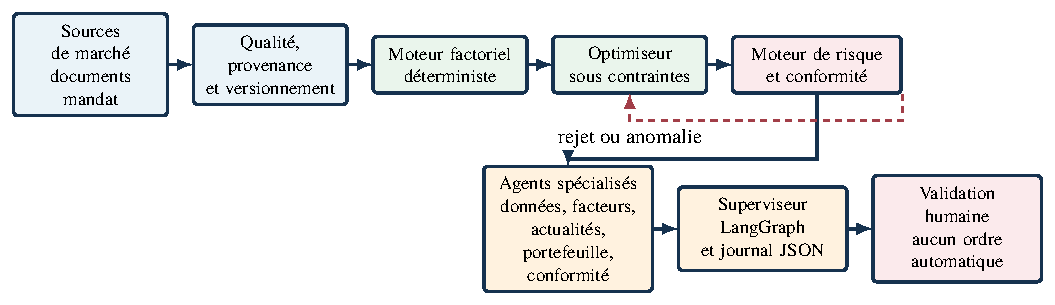
\includegraphics[width=\textwidth]{figures/schemas/architecture_globale.pdf}
\caption{Architecture cible séparant le socle quantitatif, les agents et la gouvernance.}
\label{fig:architecture-globale}
\end{figure}

\section{Rôles proposés et périmètre réalisé}

Les rôles du tableau~\ref{tab:agents-proposes} décrivent l'architecture cible : tous n'ont pas été exécutés. Les composants testés sont précisés après le tableau.

\begin{table}[H]
\centering
\caption{Rôles, permissions et limites des agents proposés.}
\label{tab:agents-proposes}
\scriptsize
\begin{adjustbox}{width=\textwidth}
\begin{tabular}{p{0.12\textwidth}p{0.20\textwidth}p{0.17\textwidth}p{0.18\textwidth}p{0.16\textwidth}p{0.17\textwidth}}
\toprule
\textbf{Agent} & \textbf{Mission} & \textbf{Outils autorisés} & \textbf{Sortie attendue} & \textbf{Interdictions} & \textbf{Conditions d'escalade} \\
\midrule
Données & Vérifier disponibilité, fraîcheur, provenance et cohérence. & APIs de données, contrôles qualité, logs. & Rapport de qualité et alertes. & Ne pas corriger silencieusement une donnée. & Donnée manquante, périmée ou incohérente. \\
Facteurs & Lancer les calculs et comparer les distributions. & Moteur déterministe, notebooks validés. & Scores, variations et anomalies. & Ne pas changer la formule ni les paramètres. & Rupture de distribution ou résultat non rejouable. \\
Actualités & Résumer nouvelles, résultats et événements macro. & OpenBB, flux autorisés, base RAG. & Synthèse sourcée et confiance. & Ne pas modifier les poids ni produire d'ordre. & Sources contradictoires ou absence de source. \\
Portefeuille & Proposer une allocation sous contraintes. & Optimiseur, mandat et coûts. & Poids cibles et attribution. & Ne pas contourner un rejet risque ou conformité. & Allocation infaisable ou contrainte violée. \\
Risque & Contrôler expositions, volatilité, drawdown et scénarios. & Moteur de risque, limites, stress tests. & Avis accepté, rejeté ou escaladé. & Ne pas relever lui-même une limite. & Limite franchie, modèle absent ou liquidité inconnue. \\
Conformité & Vérifier restrictions, documentation et séparation des rôles. & Référentiel de règles, listes, audit. & Validation ou blocage motivé. & Ne pas accorder d'exception implicite. & Règle inconnue, conflit ou trace incomplète. \\
Superviseur & Agréger les avis et préparer la revue humaine. & État complet, règles de délégation, journal. & Note de décision traçable. & Ne pas exécuter ni masquer un désaccord. & Désaccord, confiance faible ou intervention requise. \\
\bottomrule
\end{tabular}
\end{adjustbox}
\end{table}

Le workflow exécuté charge les fichiers, applique les gardes qualité et risque, puis associe un superviseur déterministe à la synthèse DeepSeek. Actualités et conformité restent proposées ; le rôle portefeuille est testé séparément dans l'extension d'allocation.

Dans le workflow de synthèse, le rapport qualité est lu après le backtest : une anomalie bloque l'accès au LLM. Le dépassement du seuil de turnover de 10\,\% ajoute une alerte d'escalade, sans interrompre la synthèse. Une sortie non conforme aux contrôles disponibles est rejetée et archivée ; le statut reste « à valider ». Les indicateurs de permission ne constituent pas une décision humaine enregistrée.

Le socle calcule rendements, poids après rendement, coûts, turnover et risque à partir de sources et paramètres identifiables, sans optimiseur institutionnel ni modèle de liquidité. Le dispositif complet prévoirait une validation humaine distincte du calcul et du contrôle qualité.

\section{Journal de décision et explicabilité}

Pour examiner une note, je repars du journal qui conserve les valeurs sources, les alertes et les permissions. Trois niveaux doivent être distingués : l'explication quantitative des calculs ; la trace des entrées, outils et règles de l'agent ; puis l'identité de la règle ou de la personne ayant validé la décision. Le texte libre demande un contrôle séparé de sa cohérence avec ces éléments.

L'extrait de la figure~\ref{fig:json-decision} provient du 30 novembre 2025. L'absence d'outil de modification des poids et d'envoi d'ordres se vérifie dans le code du workflow de synthèse ; les champs JSON en documentent la règle.

\begin{figure}[H]
\centering
\scriptsize
\begin{verbatim}
{
  "workflow": "langgraph_deterministic_supervisor",
  "date": "2025-11-30",
  "quality_ok": true,
  "risk_status": "a valider",
  "rebalance": {
    "factor_returns": {
      "Value": 0.0249981345118395,
      "Momentum": -0.0156164272534177,
      "Quality": 0.0090677798205325,
      "Low volatility": 0.0230736302539755
    },
    "net_return": 0.0103740219288315,
    "turnover": 0.0067574044008865,
    "transaction_cost": 6.757404400886513e-06,
    "target_weights": {
      "VLUE": 0.25, "MTUM": 0.25,
      "QUAL": 0.25, "USMV": 0.25
    }
  },
  "permissions": {
    "can_change_weights": false,
    "can_send_orders": false,
    "human_validation_required": true
  }
}
\end{verbatim}
\caption{Extrait réel du journal JSON produit par le prototype.}
\label{fig:json-decision}
\end{figure}

Les traces déterministes contiennent les valeurs, alertes et permissions. L'archive DeepSeek du 7 septembre 2026 ajoute le modèle et les identifiants de requête, mais pas les empreintes du prompt, des données ou le commit Git. Le code prévoit ces informations pour de nouvelles traces ; elles ne complètent pas rétroactivement l'archive. Aucune de ces sorties n'enregistre une approbation humaine effectivement réalisée.

\section{Allocation simulée et suivi des incidents}

L'extension suit une séquence explicite : indicateurs passés, proposition DeepSeek, validation indépendante, transaction simulée ou conservation des positions, puis valorisation quotidienne. Le modèle n'écrit jamais directement les quantités. Le code vérifie les poids, le turnover et les champs cités ; il revérifie les contraintes au cours d'exécution et finance les frais à partir du portefeuille.

Un rejet conserve les quantités et son motif est archivé, sans correction automatique ni nouvel appel. Le renvoi à un optimiseur avant revue humaine appartient à l'architecture proposée, pas à cette expérience. Le protocole et les résultats figurent respectivement aux sections~\ref{sec:protocole-allocation} et~\ref{sec:resultats-allocation}.

Un dispositif d'exploitation devrait suivre les citations invalides, échecs d'outils, désaccords, interventions humaines, latences et coûts, avec un responsable et une réaction définis pour chaque incident. Les seuils envisagés pour cette cible n'ont pas été calibrés sur le prototype. Les résultats mesurés de la collecte, ses rejets et ses limites sont discutés au chapitre~\ref{cap:discussion}.
